% Options for packages loaded elsewhere
\PassOptionsToPackage{unicode}{hyperref}
\PassOptionsToPackage{hyphens}{url}
%
\documentclass[
]{article}
\usepackage{amsmath,amssymb}
\usepackage{iftex}
\ifPDFTeX
  \usepackage[T1]{fontenc}
  \usepackage[utf8]{inputenc}
  \usepackage{textcomp} % provide euro and other symbols
\else % if luatex or xetex
  \usepackage{unicode-math} % this also loads fontspec
  \defaultfontfeatures{Scale=MatchLowercase}
  \defaultfontfeatures[\rmfamily]{Ligatures=TeX,Scale=1}
\fi
\usepackage{lmodern}
\ifPDFTeX\else
  % xetex/luatex font selection
\fi
% Use upquote if available, for straight quotes in verbatim environments
\IfFileExists{upquote.sty}{\usepackage{upquote}}{}
\IfFileExists{microtype.sty}{% use microtype if available
  \usepackage[]{microtype}
  \UseMicrotypeSet[protrusion]{basicmath} % disable protrusion for tt fonts
}{}
\makeatletter
\@ifundefined{KOMAClassName}{% if non-KOMA class
  \IfFileExists{parskip.sty}{%
    \usepackage{parskip}
  }{% else
    \setlength{\parindent}{0pt}
    \setlength{\parskip}{6pt plus 2pt minus 1pt}}
}{% if KOMA class
  \KOMAoptions{parskip=half}}
\makeatother
\usepackage{xcolor}
\usepackage[margin=1in]{geometry}
\usepackage{color}
\usepackage{fancyvrb}
\newcommand{\VerbBar}{|}
\newcommand{\VERB}{\Verb[commandchars=\\\{\}]}
\DefineVerbatimEnvironment{Highlighting}{Verbatim}{commandchars=\\\{\}}
% Add ',fontsize=\small' for more characters per line
\usepackage{framed}
\definecolor{shadecolor}{RGB}{248,248,248}
\newenvironment{Shaded}{\begin{snugshade}}{\end{snugshade}}
\newcommand{\AlertTok}[1]{\textcolor[rgb]{0.94,0.16,0.16}{#1}}
\newcommand{\AnnotationTok}[1]{\textcolor[rgb]{0.56,0.35,0.01}{\textbf{\textit{#1}}}}
\newcommand{\AttributeTok}[1]{\textcolor[rgb]{0.13,0.29,0.53}{#1}}
\newcommand{\BaseNTok}[1]{\textcolor[rgb]{0.00,0.00,0.81}{#1}}
\newcommand{\BuiltInTok}[1]{#1}
\newcommand{\CharTok}[1]{\textcolor[rgb]{0.31,0.60,0.02}{#1}}
\newcommand{\CommentTok}[1]{\textcolor[rgb]{0.56,0.35,0.01}{\textit{#1}}}
\newcommand{\CommentVarTok}[1]{\textcolor[rgb]{0.56,0.35,0.01}{\textbf{\textit{#1}}}}
\newcommand{\ConstantTok}[1]{\textcolor[rgb]{0.56,0.35,0.01}{#1}}
\newcommand{\ControlFlowTok}[1]{\textcolor[rgb]{0.13,0.29,0.53}{\textbf{#1}}}
\newcommand{\DataTypeTok}[1]{\textcolor[rgb]{0.13,0.29,0.53}{#1}}
\newcommand{\DecValTok}[1]{\textcolor[rgb]{0.00,0.00,0.81}{#1}}
\newcommand{\DocumentationTok}[1]{\textcolor[rgb]{0.56,0.35,0.01}{\textbf{\textit{#1}}}}
\newcommand{\ErrorTok}[1]{\textcolor[rgb]{0.64,0.00,0.00}{\textbf{#1}}}
\newcommand{\ExtensionTok}[1]{#1}
\newcommand{\FloatTok}[1]{\textcolor[rgb]{0.00,0.00,0.81}{#1}}
\newcommand{\FunctionTok}[1]{\textcolor[rgb]{0.13,0.29,0.53}{\textbf{#1}}}
\newcommand{\ImportTok}[1]{#1}
\newcommand{\InformationTok}[1]{\textcolor[rgb]{0.56,0.35,0.01}{\textbf{\textit{#1}}}}
\newcommand{\KeywordTok}[1]{\textcolor[rgb]{0.13,0.29,0.53}{\textbf{#1}}}
\newcommand{\NormalTok}[1]{#1}
\newcommand{\OperatorTok}[1]{\textcolor[rgb]{0.81,0.36,0.00}{\textbf{#1}}}
\newcommand{\OtherTok}[1]{\textcolor[rgb]{0.56,0.35,0.01}{#1}}
\newcommand{\PreprocessorTok}[1]{\textcolor[rgb]{0.56,0.35,0.01}{\textit{#1}}}
\newcommand{\RegionMarkerTok}[1]{#1}
\newcommand{\SpecialCharTok}[1]{\textcolor[rgb]{0.81,0.36,0.00}{\textbf{#1}}}
\newcommand{\SpecialStringTok}[1]{\textcolor[rgb]{0.31,0.60,0.02}{#1}}
\newcommand{\StringTok}[1]{\textcolor[rgb]{0.31,0.60,0.02}{#1}}
\newcommand{\VariableTok}[1]{\textcolor[rgb]{0.00,0.00,0.00}{#1}}
\newcommand{\VerbatimStringTok}[1]{\textcolor[rgb]{0.31,0.60,0.02}{#1}}
\newcommand{\WarningTok}[1]{\textcolor[rgb]{0.56,0.35,0.01}{\textbf{\textit{#1}}}}
\usepackage{graphicx}
\makeatletter
\def\maxwidth{\ifdim\Gin@nat@width>\linewidth\linewidth\else\Gin@nat@width\fi}
\def\maxheight{\ifdim\Gin@nat@height>\textheight\textheight\else\Gin@nat@height\fi}
\makeatother
% Scale images if necessary, so that they will not overflow the page
% margins by default, and it is still possible to overwrite the defaults
% using explicit options in \includegraphics[width, height, ...]{}
\setkeys{Gin}{width=\maxwidth,height=\maxheight,keepaspectratio}
% Set default figure placement to htbp
\makeatletter
\def\fps@figure{htbp}
\makeatother
\setlength{\emergencystretch}{3em} % prevent overfull lines
\providecommand{\tightlist}{%
  \setlength{\itemsep}{0pt}\setlength{\parskip}{0pt}}
\setcounter{secnumdepth}{-\maxdimen} % remove section numbering
\ifLuaTeX
  \usepackage{selnolig}  % disable illegal ligatures
\fi
\usepackage{bookmark}
\IfFileExists{xurl.sty}{\usepackage{xurl}}{} % add URL line breaks if available
\urlstyle{same}
\hypersetup{
  pdftitle={Homework\_DataWrangling},
  pdfauthor={Vaibhav B. Shelar},
  hidelinks,
  pdfcreator={LaTeX via pandoc}}

\title{Homework\_DataWrangling}
\author{Vaibhav B. Shelar}
\date{2025-03-19}

\begin{document}
\maketitle

\subsection{Seemless data wrangling}\label{seemless-data-wrangling}

The tidyverse is a bunch of packages and functions written by the folks
that manages Rstudio. The tidyverse builds upon base R to allow for
easier use of large datasets.h

\subsection{Install package tidyverse}\label{install-package-tidyverse}

install.packages(``tidyverse'')

\begin{Shaded}
\begin{Highlighting}[]
\FunctionTok{library}\NormalTok{(tidyverse)}
\end{Highlighting}
\end{Shaded}

\begin{verbatim}
## -- Attaching core tidyverse packages ------------------------ tidyverse 2.0.0 --
## v dplyr     1.1.4     v readr     2.1.5
## v forcats   1.0.0     v stringr   1.5.1
## v ggplot2   3.5.1     v tibble    3.2.1
## v lubridate 1.9.4     v tidyr     1.3.1
## v purrr     1.0.4     
## -- Conflicts ------------------------------------------ tidyverse_conflicts() --
## x dplyr::filter() masks stats::filter()
## x dplyr::lag()    masks stats::lag()
## i Use the conflicted package (<http://conflicted.r-lib.org/>) to force all conflicts to become errors
\end{verbatim}

\begin{Shaded}
\begin{Highlighting}[]
\NormalTok{microbiome.fungi }\OtherTok{\textless{}{-}} \FunctionTok{read.csv}\NormalTok{(}\StringTok{"Bull\_richness.csv"}\NormalTok{)}
\FunctionTok{str}\NormalTok{(microbiome.fungi)}
\end{Highlighting}
\end{Shaded}

\begin{verbatim}
## 'data.frame':    287 obs. of  16 variables:
##  $ SampleID       : chr  "Corn2017LeafObjective2Collection1T1R1CAH2" "Corn2017LeafObjective2Collection1T1R1CBA3" "Corn2017LeafObjective2Collection1T1R1CCB3" "Corn2017LeafObjective2Collection1T1R1FAC3" ...
##  $ Crop           : chr  "Corn" "Corn" "Corn" "Corn" ...
##  $ Objective      : chr  "Objective 2" "Objective 2" "Objective 2" "Objective 2" ...
##  $ Collection     : int  1 1 1 1 1 1 1 1 1 1 ...
##  $ Compartment    : chr  "Leaf" "Leaf" "Leaf" "Leaf" ...
##  $ DateSampled    : chr  "6/26/17" "6/26/17" "6/26/17" "6/26/17" ...
##  $ GrowthStage    : chr  "V6" "V6" "V6" "V6" ...
##  $ Treatment      : chr  "Conv." "Conv." "Conv." "Conv." ...
##  $ Rep            : chr  "R1" "R1" "R1" "R1" ...
##  $ Sample         : chr  "A" "B" "C" "A" ...
##  $ Fungicide      : chr  "C" "C" "C" "F" ...
##  $ Target_organism: chr  "Fungi" "Fungi" "Fungi" "Fungi" ...
##  $ Location       : chr  "Kellogg Biological Station" "Kellogg Biological Station" "Kellogg Biological Station" "Kellogg Biological Station" ...
##  $ Experiment     : chr  "LTER" "LTER" "LTER" "LTER" ...
##  $ Year           : int  2017 2017 2017 2017 2017 2017 2017 2017 2017 2017 ...
##  $ richness       : int  9 6 5 7 4 2 3 8 4 4 ...
\end{verbatim}

\subsection{select()}\label{select}

\begin{Shaded}
\begin{Highlighting}[]
\NormalTok{microbiome.fungi2 }\OtherTok{\textless{}{-}} \FunctionTok{select}\NormalTok{(microbiome.fungi, SampleID, Crop, Compartment}\SpecialCharTok{:}\NormalTok{Fungicide, richness)}
\end{Highlighting}
\end{Shaded}

\subsection{filter()}\label{filter}

\begin{Shaded}
\begin{Highlighting}[]
\FunctionTok{head}\NormalTok{(}\FunctionTok{filter}\NormalTok{(microbiome.fungi2, Treatment }\SpecialCharTok{==} \StringTok{"Conv."}\NormalTok{))}
\end{Highlighting}
\end{Shaded}

\begin{verbatim}
##                                    SampleID Crop Compartment DateSampled
## 1 Corn2017LeafObjective2Collection1T1R1CAH2 Corn        Leaf     6/26/17
## 2 Corn2017LeafObjective2Collection1T1R1CBA3 Corn        Leaf     6/26/17
## 3 Corn2017LeafObjective2Collection1T1R1CCB3 Corn        Leaf     6/26/17
## 4 Corn2017LeafObjective2Collection1T1R1FAC3 Corn        Leaf     6/26/17
## 5 Corn2017LeafObjective2Collection1T1R1FBD3 Corn        Leaf     6/26/17
## 6 Corn2017LeafObjective2Collection1T1R1FCE3 Corn        Leaf     6/26/17
##   GrowthStage Treatment Rep Sample Fungicide richness
## 1          V6     Conv.  R1      A         C        9
## 2          V6     Conv.  R1      B         C        6
## 3          V6     Conv.  R1      C         C        5
## 4          V6     Conv.  R1      A         F        7
## 5          V6     Conv.  R1      B         F        4
## 6          V6     Conv.  R1      C         F        2
\end{verbatim}

\begin{Shaded}
\begin{Highlighting}[]
\CommentTok{\# A more complex using \& }
\FunctionTok{head}\NormalTok{(}\FunctionTok{filter}\NormalTok{(microbiome.fungi2, Treatment }\SpecialCharTok{==} \StringTok{"Conv."} \SpecialCharTok{\&}\NormalTok{ Fungicide }\SpecialCharTok{==} \StringTok{"C"}\NormalTok{))}
\end{Highlighting}
\end{Shaded}

\begin{verbatim}
##                                    SampleID Crop Compartment DateSampled
## 1 Corn2017LeafObjective2Collection1T1R1CAH2 Corn        Leaf     6/26/17
## 2 Corn2017LeafObjective2Collection1T1R1CBA3 Corn        Leaf     6/26/17
## 3 Corn2017LeafObjective2Collection1T1R1CCB3 Corn        Leaf     6/26/17
## 4 Corn2017LeafObjective2Collection1T1R2CAF3 Corn        Leaf     6/26/17
## 5 Corn2017LeafObjective2Collection1T1R2CBG3 Corn        Leaf     6/26/17
## 6 Corn2017LeafObjective2Collection1T1R2CCH3 Corn        Leaf     6/26/17
##   GrowthStage Treatment Rep Sample Fungicide richness
## 1          V6     Conv.  R1      A         C        9
## 2          V6     Conv.  R1      B         C        6
## 3          V6     Conv.  R1      C         C        5
## 4          V6     Conv.  R2      A         C        3
## 5          V6     Conv.  R2      B         C        8
## 6          V6     Conv.  R2      C         C        4
\end{verbatim}

\begin{Shaded}
\begin{Highlighting}[]
\CommentTok{\# Another more complex using or |}
\FunctionTok{head}\NormalTok{(}\FunctionTok{filter}\NormalTok{(microbiome.fungi2, Sample }\SpecialCharTok{==} \StringTok{"A"} \SpecialCharTok{|}\NormalTok{ Sample }\SpecialCharTok{==} \StringTok{"B"}\NormalTok{)) }\CommentTok{\#Sample A or B}
\end{Highlighting}
\end{Shaded}

\begin{verbatim}
##                                    SampleID Crop Compartment DateSampled
## 1 Corn2017LeafObjective2Collection1T1R1CAH2 Corn        Leaf     6/26/17
## 2 Corn2017LeafObjective2Collection1T1R1CBA3 Corn        Leaf     6/26/17
## 3 Corn2017LeafObjective2Collection1T1R1FAC3 Corn        Leaf     6/26/17
## 4 Corn2017LeafObjective2Collection1T1R1FBD3 Corn        Leaf     6/26/17
## 5 Corn2017LeafObjective2Collection1T1R2CAF3 Corn        Leaf     6/26/17
## 6 Corn2017LeafObjective2Collection1T1R2CBG3 Corn        Leaf     6/26/17
##   GrowthStage Treatment Rep Sample Fungicide richness
## 1          V6     Conv.  R1      A         C        9
## 2          V6     Conv.  R1      B         C        6
## 3          V6     Conv.  R1      A         F        7
## 4          V6     Conv.  R1      B         F        4
## 5          V6     Conv.  R2      A         C        3
## 6          V6     Conv.  R2      B         C        8
\end{verbatim}

\subsection{mutate()}\label{mutate}

It allows us to quickly create new columns

\begin{Shaded}
\begin{Highlighting}[]
\NormalTok{microbiome.fungi2}\SpecialCharTok{$}\NormalTok{logRich }\OtherTok{\textless{}{-}} \FunctionTok{log}\NormalTok{(microbiome.fungi2}\SpecialCharTok{$}\NormalTok{richness)}

\CommentTok{\# Create a new column called logRich}
\FunctionTok{head}\NormalTok{(}\FunctionTok{mutate}\NormalTok{(microbiome.fungi2, }\AttributeTok{logRich =} \FunctionTok{log}\NormalTok{(richness)))}
\end{Highlighting}
\end{Shaded}

\begin{verbatim}
##                                    SampleID Crop Compartment DateSampled
## 1 Corn2017LeafObjective2Collection1T1R1CAH2 Corn        Leaf     6/26/17
## 2 Corn2017LeafObjective2Collection1T1R1CBA3 Corn        Leaf     6/26/17
## 3 Corn2017LeafObjective2Collection1T1R1CCB3 Corn        Leaf     6/26/17
## 4 Corn2017LeafObjective2Collection1T1R1FAC3 Corn        Leaf     6/26/17
## 5 Corn2017LeafObjective2Collection1T1R1FBD3 Corn        Leaf     6/26/17
## 6 Corn2017LeafObjective2Collection1T1R1FCE3 Corn        Leaf     6/26/17
##   GrowthStage Treatment Rep Sample Fungicide richness   logRich
## 1          V6     Conv.  R1      A         C        9 2.1972246
## 2          V6     Conv.  R1      B         C        6 1.7917595
## 3          V6     Conv.  R1      C         C        5 1.6094379
## 4          V6     Conv.  R1      A         F        7 1.9459101
## 5          V6     Conv.  R1      B         F        4 1.3862944
## 6          V6     Conv.  R1      C         F        2 0.6931472
\end{verbatim}

\begin{Shaded}
\begin{Highlighting}[]
\CommentTok{\# Creating a new column which combines Crop and Treatment}
\FunctionTok{head}\NormalTok{(}\FunctionTok{mutate}\NormalTok{(microbiome.fungi2, }\AttributeTok{Crop\_Treatment =} \FunctionTok{paste}\NormalTok{(Crop, Treatment)))}
\end{Highlighting}
\end{Shaded}

\begin{verbatim}
##                                    SampleID Crop Compartment DateSampled
## 1 Corn2017LeafObjective2Collection1T1R1CAH2 Corn        Leaf     6/26/17
## 2 Corn2017LeafObjective2Collection1T1R1CBA3 Corn        Leaf     6/26/17
## 3 Corn2017LeafObjective2Collection1T1R1CCB3 Corn        Leaf     6/26/17
## 4 Corn2017LeafObjective2Collection1T1R1FAC3 Corn        Leaf     6/26/17
## 5 Corn2017LeafObjective2Collection1T1R1FBD3 Corn        Leaf     6/26/17
## 6 Corn2017LeafObjective2Collection1T1R1FCE3 Corn        Leaf     6/26/17
##   GrowthStage Treatment Rep Sample Fungicide richness   logRich Crop_Treatment
## 1          V6     Conv.  R1      A         C        9 2.1972246     Corn Conv.
## 2          V6     Conv.  R1      B         C        6 1.7917595     Corn Conv.
## 3          V6     Conv.  R1      C         C        5 1.6094379     Corn Conv.
## 4          V6     Conv.  R1      A         F        7 1.9459101     Corn Conv.
## 5          V6     Conv.  R1      B         F        4 1.3862944     Corn Conv.
## 6          V6     Conv.  R1      C         F        2 0.6931472     Corn Conv.
\end{verbatim}

\subsubsection{the pipe `\%\textgreater\%'}\label{the-pipe}

\begin{Shaded}
\begin{Highlighting}[]
\FunctionTok{library}\NormalTok{(dplyr)}
\end{Highlighting}
\end{Shaded}

\begin{Shaded}
\begin{Highlighting}[]
\NormalTok{microbiome.fungi }\SpecialCharTok{\%\textgreater{}\%}
  \FunctionTok{select}\NormalTok{(SampleID, Crop, Compartment}\SpecialCharTok{:}\NormalTok{Fungicide, richness) }\SpecialCharTok{\%\textgreater{}\%}  \CommentTok{\# selecting columns}
  \FunctionTok{filter}\NormalTok{(Treatment }\SpecialCharTok{==} \StringTok{"Conv."}\NormalTok{) }\SpecialCharTok{\%\textgreater{}\%}  \CommentTok{\# subsetting to only include the conventional treatments}
  \FunctionTok{mutate}\NormalTok{(}\AttributeTok{logRich =} \FunctionTok{log}\NormalTok{(richness)) }\SpecialCharTok{\%\textgreater{}\%}  \CommentTok{\# creating new column of the log richness}
  \FunctionTok{head}\NormalTok{()  }\CommentTok{\# displaying the forst six rows}
\end{Highlighting}
\end{Shaded}

\begin{verbatim}
##                                    SampleID Crop Compartment DateSampled
## 1 Corn2017LeafObjective2Collection1T1R1CAH2 Corn        Leaf     6/26/17
## 2 Corn2017LeafObjective2Collection1T1R1CBA3 Corn        Leaf     6/26/17
## 3 Corn2017LeafObjective2Collection1T1R1CCB3 Corn        Leaf     6/26/17
## 4 Corn2017LeafObjective2Collection1T1R1FAC3 Corn        Leaf     6/26/17
## 5 Corn2017LeafObjective2Collection1T1R1FBD3 Corn        Leaf     6/26/17
## 6 Corn2017LeafObjective2Collection1T1R1FCE3 Corn        Leaf     6/26/17
##   GrowthStage Treatment Rep Sample Fungicide richness   logRich
## 1          V6     Conv.  R1      A         C        9 2.1972246
## 2          V6     Conv.  R1      B         C        6 1.7917595
## 3          V6     Conv.  R1      C         C        5 1.6094379
## 4          V6     Conv.  R1      A         F        7 1.9459101
## 5          V6     Conv.  R1      B         F        4 1.3862944
## 6          V6     Conv.  R1      C         F        2 0.6931472
\end{verbatim}

\subsubsection{`summerise()'}\label{summerise}

Use to find the mean, standard deviations/errors

\begin{Shaded}
\begin{Highlighting}[]
\NormalTok{microbiome.fungi }\SpecialCharTok{\%\textgreater{}\%}
  \FunctionTok{select}\NormalTok{(SampleID, Crop, Compartment}\SpecialCharTok{:}\NormalTok{Fungicide, richness) }\SpecialCharTok{\%\textgreater{}\%}  \CommentTok{\# selecting columns}
  \FunctionTok{filter}\NormalTok{(Treatment }\SpecialCharTok{==} \StringTok{"Conv."}\NormalTok{) }\SpecialCharTok{\%\textgreater{}\%}  \CommentTok{\# subsetting to only include the conventional treatments}
  \FunctionTok{mutate}\NormalTok{(}\AttributeTok{logRich =} \FunctionTok{log}\NormalTok{(richness)) }\SpecialCharTok{\%\textgreater{}\%}  \CommentTok{\# creating new column of the log richness}
  \FunctionTok{summarise}\NormalTok{(}\AttributeTok{Mean.rich =} \FunctionTok{mean}\NormalTok{(logRich))  }\CommentTok{\#Calculating overall mean log richness within the conventionally managed treatments }
\end{Highlighting}
\end{Shaded}

\begin{verbatim}
##   Mean.rich
## 1  2.304395
\end{verbatim}

\subsubsection{`group\_by()'}\label{group_by}

\begin{Shaded}
\begin{Highlighting}[]
\NormalTok{microbiome.fungi }\SpecialCharTok{\%\textgreater{}\%}
  \FunctionTok{select}\NormalTok{(SampleID, Crop, Compartment}\SpecialCharTok{:}\NormalTok{Fungicide, richness) }\SpecialCharTok{\%\textgreater{}\%}  \CommentTok{\# selecting columns}
  \FunctionTok{filter}\NormalTok{(Treatment }\SpecialCharTok{==} \StringTok{"Conv."}\NormalTok{) }\SpecialCharTok{\%\textgreater{}\%}  \CommentTok{\# subsetting to only include the conventional treatments}
  \FunctionTok{mutate}\NormalTok{(}\AttributeTok{logRich =} \FunctionTok{log}\NormalTok{(richness)) }\SpecialCharTok{\%\textgreater{}\%}  \CommentTok{\# creating new column of the log richness}
  \FunctionTok{summarise}\NormalTok{(}\AttributeTok{Mean.rich =} \FunctionTok{mean}\NormalTok{(logRich),  }\CommentTok{\#Calculating the mean richness, stdeviation, adn standard error}
            \AttributeTok{n =} \FunctionTok{n}\NormalTok{(),}
            \AttributeTok{sd.dev =} \FunctionTok{sd}\NormalTok{(logRich)) }\SpecialCharTok{\%\textgreater{}\%} 
  \FunctionTok{mutate}\NormalTok{(}\AttributeTok{std.err =}\NormalTok{ sd.dev}\SpecialCharTok{/}\FunctionTok{sqrt}\NormalTok{(n))}
\end{Highlighting}
\end{Shaded}

\begin{verbatim}
##   Mean.rich   n    sd.dev   std.err
## 1  2.304395 144 0.7024667 0.0585389
\end{verbatim}

\subsubsection{Connecting to plotting}\label{connecting-to-plotting}

\begin{Shaded}
\begin{Highlighting}[]
\FunctionTok{library}\NormalTok{(ggplot2)}
\NormalTok{microbiome.fungi }\SpecialCharTok{\%\textgreater{}\%}
  \FunctionTok{select}\NormalTok{(SampleID, Crop, Compartment}\SpecialCharTok{:}\NormalTok{Fungicide, richness) }\SpecialCharTok{\%\textgreater{}\%}  \CommentTok{\# selecting columns}
  \FunctionTok{group\_by}\NormalTok{(Treatment, Fungicide) }\SpecialCharTok{\%\textgreater{}\%}  \CommentTok{\# grouping by treatment and fungicide to later calculate summary stats by group}
  \FunctionTok{mutate}\NormalTok{(}\AttributeTok{logRich =} \FunctionTok{log}\NormalTok{(richness)) }\SpecialCharTok{\%\textgreater{}\%} \CommentTok{\# creating a new column of the log richness }
  \FunctionTok{summarise}\NormalTok{(}\AttributeTok{Mean.rich =} \FunctionTok{mean}\NormalTok{(logRich), }\CommentTok{\# calculating the mean richness, stdeviation, and standard error }
            \AttributeTok{n =} \FunctionTok{n}\NormalTok{(),}
            \AttributeTok{sd.dev =} \FunctionTok{sd}\NormalTok{(logRich)) }\SpecialCharTok{\%\textgreater{}\%}
  \FunctionTok{mutate}\NormalTok{(}\AttributeTok{std.err =}\NormalTok{ sd.dev}\SpecialCharTok{/}\FunctionTok{sqrt}\NormalTok{(n)) }\SpecialCharTok{\%\textgreater{}\%} 
  \FunctionTok{ggplot}\NormalTok{(}\FunctionTok{aes}\NormalTok{(}\AttributeTok{x =}\NormalTok{ Fungicide, }\AttributeTok{y =}\NormalTok{ Mean.rich)) }\SpecialCharTok{+} \CommentTok{\# adding in a ggplot }
  \FunctionTok{geom\_bar}\NormalTok{(}\AttributeTok{stat =} \StringTok{"identity"}\NormalTok{) }\SpecialCharTok{+}
  \FunctionTok{geom\_errorbar}\NormalTok{(}\FunctionTok{aes}\NormalTok{(}\AttributeTok{x =}\NormalTok{ Fungicide, }\AttributeTok{ymin =}\NormalTok{ Mean.rich }\SpecialCharTok{{-}}\NormalTok{ std.err, }\AttributeTok{ymax =}\NormalTok{ Mean.rich }\SpecialCharTok{+}\NormalTok{ std.err), }\AttributeTok{width =} \FloatTok{0.4}\NormalTok{) }\SpecialCharTok{+} 
  \FunctionTok{theme\_minimal}\NormalTok{() }\SpecialCharTok{+} 
  \FunctionTok{xlab}\NormalTok{(}\StringTok{""}\NormalTok{) }\SpecialCharTok{+}
  \FunctionTok{ylab}\NormalTok{(}\StringTok{"Log Richness"}\NormalTok{) }\SpecialCharTok{+}
  \FunctionTok{facet\_wrap}\NormalTok{(}\SpecialCharTok{\textasciitilde{}}\NormalTok{Treatment)}
\end{Highlighting}
\end{Shaded}

\begin{verbatim}
## `summarise()` has grouped output by 'Treatment'. You can override using the
## `.groups` argument.
\end{verbatim}

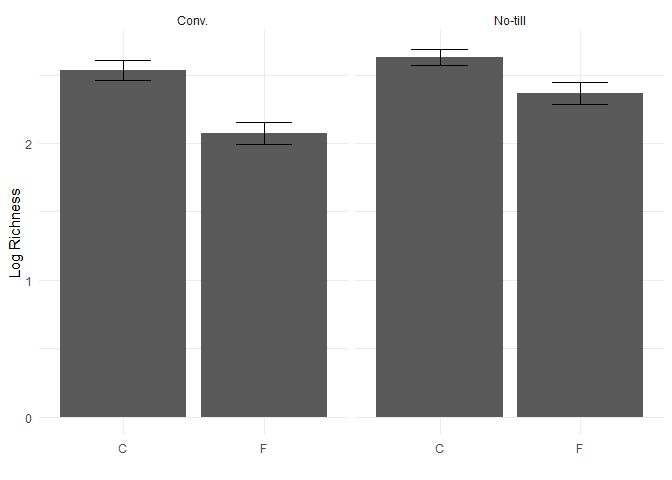
\includegraphics{Homework_DataWrangling_files/figure-latex/unnamed-chunk-10-1.pdf}

\subsubsection{Joining}\label{joining}

\begin{Shaded}
\begin{Highlighting}[]
\CommentTok{\# selecting just the richness and sample id }
\NormalTok{richness }\OtherTok{\textless{}{-}}\NormalTok{ microbiome.fungi }\SpecialCharTok{\%\textgreater{}\%} 
\FunctionTok{select}\NormalTok{(SampleID, richness)  }

\CommentTok{\# selecting the columns that dont include the richness}
\NormalTok{metadata }\OtherTok{\textless{}{-}}\NormalTok{ microbiome.fungi }\SpecialCharTok{\%\textgreater{}\%} 
\FunctionTok{select}\NormalTok{(SampleID, Fungicide, Crop, Compartment, GrowthStage, Treatment, Rep, Sample)}

\FunctionTok{head}\NormalTok{(metadata)}
\end{Highlighting}
\end{Shaded}

\begin{verbatim}
##                                    SampleID Fungicide Crop Compartment
## 1 Corn2017LeafObjective2Collection1T1R1CAH2         C Corn        Leaf
## 2 Corn2017LeafObjective2Collection1T1R1CBA3         C Corn        Leaf
## 3 Corn2017LeafObjective2Collection1T1R1CCB3         C Corn        Leaf
## 4 Corn2017LeafObjective2Collection1T1R1FAC3         F Corn        Leaf
## 5 Corn2017LeafObjective2Collection1T1R1FBD3         F Corn        Leaf
## 6 Corn2017LeafObjective2Collection1T1R1FCE3         F Corn        Leaf
##   GrowthStage Treatment Rep Sample
## 1          V6     Conv.  R1      A
## 2          V6     Conv.  R1      B
## 3          V6     Conv.  R1      C
## 4          V6     Conv.  R1      A
## 5          V6     Conv.  R1      B
## 6          V6     Conv.  R1      C
\end{verbatim}

\begin{Shaded}
\begin{Highlighting}[]
\FunctionTok{head}\NormalTok{(richness)}
\end{Highlighting}
\end{Shaded}

\begin{verbatim}
##                                    SampleID richness
## 1 Corn2017LeafObjective2Collection1T1R1CAH2        9
## 2 Corn2017LeafObjective2Collection1T1R1CBA3        6
## 3 Corn2017LeafObjective2Collection1T1R1CCB3        5
## 4 Corn2017LeafObjective2Collection1T1R1FAC3        7
## 5 Corn2017LeafObjective2Collection1T1R1FBD3        4
## 6 Corn2017LeafObjective2Collection1T1R1FCE3        2
\end{verbatim}

\begin{Shaded}
\begin{Highlighting}[]
\FunctionTok{head}\NormalTok{(}\FunctionTok{left\_join}\NormalTok{(metadata, richness, }\AttributeTok{by =} \StringTok{"SampleID"}\NormalTok{)) }\CommentTok{\# adding the richness data to the metadata based on the common column of sampleID}
\end{Highlighting}
\end{Shaded}

\begin{verbatim}
##                                    SampleID Fungicide Crop Compartment
## 1 Corn2017LeafObjective2Collection1T1R1CAH2         C Corn        Leaf
## 2 Corn2017LeafObjective2Collection1T1R1CBA3         C Corn        Leaf
## 3 Corn2017LeafObjective2Collection1T1R1CCB3         C Corn        Leaf
## 4 Corn2017LeafObjective2Collection1T1R1FAC3         F Corn        Leaf
## 5 Corn2017LeafObjective2Collection1T1R1FBD3         F Corn        Leaf
## 6 Corn2017LeafObjective2Collection1T1R1FCE3         F Corn        Leaf
##   GrowthStage Treatment Rep Sample richness
## 1          V6     Conv.  R1      A        9
## 2          V6     Conv.  R1      B        6
## 3          V6     Conv.  R1      C        5
## 4          V6     Conv.  R1      A        7
## 5          V6     Conv.  R1      B        4
## 6          V6     Conv.  R1      C        2
\end{verbatim}

\subsubsection{Pivoting}\label{pivoting}

Pivoting is also useful for converting from wide to long format and back
again. We can do this with `pivot\_longer()' and `pivot\_wider()'

\begin{Shaded}
\begin{Highlighting}[]
\NormalTok{microbiome.fungi }\SpecialCharTok{\%\textgreater{}\%}
  \FunctionTok{select}\NormalTok{(SampleID, Crop, Compartment}\SpecialCharTok{:}\NormalTok{Fungicide, richness) }\SpecialCharTok{\%\textgreater{}\%}
   \FunctionTok{group\_by}\NormalTok{(Treatment, Fungicide) }\SpecialCharTok{\%\textgreater{}\%}  \CommentTok{\# grouping by treatment and fungicide to later calculate summary stats by group}
  \FunctionTok{summarise}\NormalTok{(}\AttributeTok{Mean =} \FunctionTok{mean}\NormalTok{(richness))  }\CommentTok{\# Calculate the mean per Treatment and fungicide}
\end{Highlighting}
\end{Shaded}

\begin{verbatim}
## `summarise()` has grouped output by 'Treatment'. You can override using the
## `.groups` argument.
\end{verbatim}

\begin{verbatim}
## # A tibble: 4 x 3
## # Groups:   Treatment [2]
##   Treatment Fungicide  Mean
##   <chr>     <chr>     <dbl>
## 1 Conv.     C         14.6 
## 2 Conv.     F          9.75
## 3 No-till   C         15.4 
## 4 No-till   F         13.1
\end{verbatim}

\section{Wide format -dets the values within the fungicide column into
column
names}\label{wide-format--dets-the-values-within-the-fungicide-column-into-column-names}

\begin{Shaded}
\begin{Highlighting}[]
\NormalTok{microbiome.fungi }\SpecialCharTok{\%\textgreater{}\%}
  \FunctionTok{select}\NormalTok{(SampleID, Crop, Compartment}\SpecialCharTok{:}\NormalTok{Fungicide, richness) }\SpecialCharTok{\%\textgreater{}\%}
   \FunctionTok{group\_by}\NormalTok{(Treatment, Fungicide) }\SpecialCharTok{\%\textgreater{}\%}  \CommentTok{\# grouping by treatment and fungicide to later calculate summary stats by group}
  \FunctionTok{summarise}\NormalTok{(}\AttributeTok{Mean =} \FunctionTok{mean}\NormalTok{(richness)) }\SpecialCharTok{\%\textgreater{}\%}  \CommentTok{\# Calculate the mean per Treatment and fungicide}
  \FunctionTok{pivot\_wider}\NormalTok{(}\AttributeTok{names\_from =}\NormalTok{ Fungicide, }\AttributeTok{values\_from =}\NormalTok{ Mean) }\CommentTok{\# pivot to wide format}
\end{Highlighting}
\end{Shaded}

\begin{verbatim}
## `summarise()` has grouped output by 'Treatment'. You can override using the
## `.groups` argument.
\end{verbatim}

\begin{verbatim}
## # A tibble: 2 x 3
## # Groups:   Treatment [2]
##   Treatment     C     F
##   <chr>     <dbl> <dbl>
## 1 Conv.      14.6  9.75
## 2 No-till    15.4 13.1
\end{verbatim}

\begin{Shaded}
\begin{Highlighting}[]
\NormalTok{microbiome.fungi }\SpecialCharTok{\%\textgreater{}\%}
  \FunctionTok{select}\NormalTok{(SampleID, Crop, Compartment}\SpecialCharTok{:}\NormalTok{Fungicide, richness) }\SpecialCharTok{\%\textgreater{}\%}
   \FunctionTok{group\_by}\NormalTok{(Treatment, Fungicide) }\SpecialCharTok{\%\textgreater{}\%}  \CommentTok{\# grouping by treatment and fungicide to later calculate summary stats by group}
  \FunctionTok{summarise}\NormalTok{(}\AttributeTok{Mean =} \FunctionTok{mean}\NormalTok{(richness)) }\SpecialCharTok{\%\textgreater{}\%}  \CommentTok{\# Calculate the mean per Treatment and fungicide}
  \FunctionTok{pivot\_wider}\NormalTok{(}\AttributeTok{names\_from =}\NormalTok{ Fungicide, }\AttributeTok{values\_from =}\NormalTok{ Mean) }\SpecialCharTok{\%\textgreater{}\%} \CommentTok{\# pivot to wide format}
  \FunctionTok{mutate}\NormalTok{(}\AttributeTok{diff.fungicide =}\NormalTok{ C }\SpecialCharTok{{-}}\NormalTok{ F) }\CommentTok{\# calculate the difference between means}
\end{Highlighting}
\end{Shaded}

\begin{verbatim}
## `summarise()` has grouped output by 'Treatment'. You can override using the
## `.groups` argument.
\end{verbatim}

\begin{verbatim}
## # A tibble: 2 x 4
## # Groups:   Treatment [2]
##   Treatment     C     F diff.fungicide
##   <chr>     <dbl> <dbl>          <dbl>
## 1 Conv.      14.6  9.75           4.89
## 2 No-till    15.4 13.1            2.32
\end{verbatim}

\begin{Shaded}
\begin{Highlighting}[]
\NormalTok{microbiome.fungi }\SpecialCharTok{\%\textgreater{}\%}
  \FunctionTok{select}\NormalTok{(SampleID, Crop, Compartment}\SpecialCharTok{:}\NormalTok{Fungicide, richness) }\SpecialCharTok{\%\textgreater{}\%} \CommentTok{\# selecting columns  }
  \FunctionTok{group\_by}\NormalTok{(Treatment, Fungicide) }\SpecialCharTok{\%\textgreater{}\%} \CommentTok{\# grouping by treatment and fungicide to later calculate summary stats by group}
  \FunctionTok{summarise}\NormalTok{(}\AttributeTok{Mean =} \FunctionTok{mean}\NormalTok{(richness)) }\SpecialCharTok{\%\textgreater{}\%} \CommentTok{\# calculates the mean per Treatment and Fungicide }
  \FunctionTok{pivot\_wider}\NormalTok{(}\AttributeTok{names\_from =}\NormalTok{ Fungicide, }\AttributeTok{values\_from =}\NormalTok{ Mean) }\SpecialCharTok{\%\textgreater{}\%} \CommentTok{\# pivot to wide format}
  \FunctionTok{mutate}\NormalTok{(}\AttributeTok{diff.fungicide =}\NormalTok{ C }\SpecialCharTok{{-}}\NormalTok{ F) }\SpecialCharTok{\%\textgreater{}\%}  \CommentTok{\# calculate the difference between the means. }
  \FunctionTok{ggplot}\NormalTok{(}\FunctionTok{aes}\NormalTok{(}\AttributeTok{x =}\NormalTok{ Treatment, }\AttributeTok{y =}\NormalTok{ diff.fungicide)) }\SpecialCharTok{+} \CommentTok{\# Plot it }
  \FunctionTok{geom\_col}\NormalTok{() }\SpecialCharTok{+}
  \FunctionTok{theme\_minimal}\NormalTok{() }\SpecialCharTok{+}
  \FunctionTok{xlab}\NormalTok{(}\StringTok{""}\NormalTok{) }\SpecialCharTok{+}
  \FunctionTok{ylab}\NormalTok{(}\StringTok{"Difference in average species richness"}\NormalTok{)}
\end{Highlighting}
\end{Shaded}

\begin{verbatim}
## `summarise()` has grouped output by 'Treatment'. You can override using the
## `.groups` argument.
\end{verbatim}

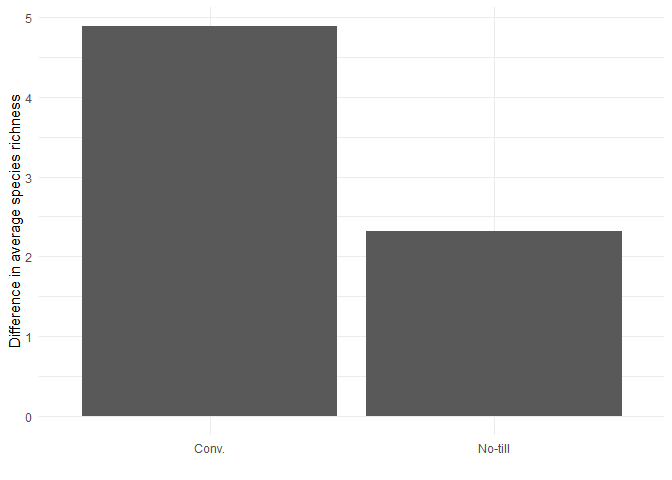
\includegraphics{Homework_DataWrangling_files/figure-latex/unnamed-chunk-15-1.pdf}

\end{document}
